
\documentclass[10pt,journal,compsoc]{IEEEtran}
\usepackage{listings}
\usepackage[pdftex]{graphicx}    
\usepackage{cite}

\usepackage{color}

\definecolor{mygreen}{rgb}{0,0.6,0}
\definecolor{mygray}{rgb}{0.5,0.5,0.5}
\definecolor{mymauve}{rgb}{0.58,0,0.82}

\lstset{ 
  backgroundcolor=\color{white},   % choose the background color; you must add \usepackage{color} or \usepackage{xcolor}; should come as last argument
  basicstyle=\footnotesize,        % the size of the fonts that are used for the code
  breakatwhitespace=false,         % sets if automatic breaks should only happen at whitespace
  breaklines=true,                 % sets automatic line breaking
  captionpos=b,                    % sets the caption-position to bottom
  commentstyle=\color{mygreen},    % comment style
  deletekeywords={...},            % if you want to delete keywords from the given language
  escapeinside={\%*}{*)},          % if you want to add LaTeX within your code
  extendedchars=true,              % lets you use non-ASCII characters; for 8-bits encodings only, does not work with UTF-8
  frame=single,	                   % adds a frame around the code
  keepspaces=true,                 % keeps spaces in text, useful for keeping indentation of code (possibly needs columns=flexible)
  keywordstyle=\color{blue},       % keyword style
  language=Octave,                 % the language of the code
  morekeywords={*,...},            % if you want to add more keywords to the set
  numbers=left,                    % where to put the line-numbers; possible values are (none, left, right)
  numbersep=5pt,                   % how far the line-numbers are from the code
  numberstyle=\tiny\color{mygray}, % the style that is used for the line-numbers
  rulecolor=\color{black},         % if not set, the frame-color may be changed on line-breaks within not-black text (e.g. comments (green here))
  showspaces=false,                % show spaces everywhere adding particular underscores; it overrides 'showstringspaces'
  showstringspaces=false,          % underline spaces within strings only
  showtabs=false,                  % show tabs within strings adding particular underscores
  stepnumber=2,                    % the step between two line-numbers. If it's 1, each line will be numbered
  stringstyle=\color{mymauve},     % string literal style
  tabsize=2,	                   % sets default tabsize to 2 spaces
  title=\lstname                   % show the filename of files included with \lstinputlisting; also try caption instead of title
}

\hyphenation{op-tical net-works semi-conduc-tor}


\begin{document}

\title{Deep Neural Network Reinforcement Learning of an Robot arm }

\author{Jung, Myoungki}

\markboth{SLAM project, Robotics Nanodegree Program, Udacity}%
{}
\IEEEtitleabstractindextext{%

\begin{abstract}
Self teaching Robots have been always a dream for robotisists and scifi fans in the world. Reinforcement learning algorithms with deep neural network techonologys opens up new horizon to these ideas and enables many robots able to learn from the environment.
Apperance of Alpha GO \cite{Fu2016} indeed shed new fresh lights on this old research field and now this topic is one of the most active field of study in artificial intellegence since then. The purpose of this report is to show an application of an end to end reinforcment learning with neural newtork to the robotics field.
\end{abstract}

% Note that keywords are not normally used for peerreview papers.
\begin{IEEEkeywords}
Robot Arm, IEEEtran, Udacity, RL, 3DOF, DQN.
\end{IEEEkeywords}}

\maketitle
\IEEEdisplaynontitleabstractindextext
\IEEEpeerreviewmaketitle
\section{Introduction}
\label{sec:introduction}

\IEEEPARstart{R}{inforcement} learning always has been in the scholars hot topic well before Deepminds' atari game mastering \cite{Mirowski2016}, even before the TD Gammon game shipped in a desktop. With advancement of deep neaural networks, its application to reinforcment learning enables researchers to overcome its previous theoretical limits and chalanges, high dimensional problems, speed of convergence and many more, which are the reasons why RL has been in research feild for a long time but not much progress like other topics until recently. Alphago Zero\cite{Hassabis2017}, an agent learning the game of Go without any human game play data unlike its predecessor, shows how eficient reinforcement learning can be compared to humans' learning by mastering the game within months and play more intellegent than any human gamer in the world in that short time.

\section{Implementation}
\subsection{Set up}
Reward functions were coded in the cpp plugin file as shown in the listing \ref{list:RewardFunction0} and \ref{list:IntermediaryRewardFunction}.
The contact were determined by the \verb!ArmPlugin::onCollisionMsg!, a callback function of contact subscription shown in listing \ref{list:Load}.

\begin{lstlisting}[language=C++, caption={ArmPlugin::Load},label={list:Load}]
void ArmPlugin::Load(physics::ModelPtr _parent, sdf::ElementPtr /*_sdf*/)
{
      printf("ArmPlugin::Load('%s')\n", _parent->GetName().c_str());
      
      //pointer to the model
      this->model = _parent;
      this->j2_controller = new physics::JointController(model);
      
      // camera communication node
      cameraNode->Init();
      cameraSub = cameraNode->Subscribe("/gazebo/" WORLD_NAME "/camera/link/camera/image", &ArmPlugin::onCameraMsg, this);
      
      // collision detection node
      collisionNode->Init();
      collisionSub = collisionNode->Subscribe("/gazebo/" WORLD_NAME "/" PROP_NAME "/tube_link/my_contact", &ArmPlugin::onCollisionMsg, this);
      
      // event update
      this->updateConnection = event::Events::ConnectWorldUpdateBegin(boost::bind(&ArmPlugin::OnUpdate, this, _1));
}
\end{lstlisting}

\subsection{Reward function}
The message from contacts topic was decoded and compared by \verb!strcmp! function and determined the reward or penalty. If contacted items are tube and \verb!gripper_link!, then the agent is rewared 12 points and other cases the agents penalised for -8 points.

\begin{lstlisting}[language=C++, caption={Reward Function},label={list:RewardFunction0}]
// Define Reward Parameters
#define REWARD_WIN   12.0f
#define REWARD_LOSS -8.0f
#define REWARD_MULTIPLIER 10.0f

#define COLLISION_FILTER "ground_plane::link::collision"
#define COLLISION_ITEM   "tube::tube_link::tube_collision"
#define COLLISION_POINT  "arm::gripperbase::gripper_link"

// onCollisionMsg
void ArmPlugin::onCollisionMsg(ConstContactsPtr &contacts)
{
      if( testAnimation ) return;
      
      for (int i = 0; i < contacts->contact_size(); ++i)
      {
            if( strcmp(contacts->contact(i).collision2().c_str(), COLLISION_FILTER) == 0 ) continue;
            
            std::cout << "Collision between[" << contacts->contact(i).collision1() << "] and [" << contacts->contact(i).collision2() << "]\n";
            
            if((strcmp(contacts->contact(i).collision1().c_str(), COLLISION_ITEM) == 0) && (strcmp(contacts->contact(i).collision2().c_str(), COLLISION_POINT) == 0))
            {
            rewardHistory = REWARD_WIN;
                  newReward  = true;
                  endEpisode = true;
                  return;
            }
            else {
                  rewardHistory = REWARD_LOSS;
                  newReward  = true;
                  endEpisode = true;
            }
      }
}
\end{lstlisting}
The agent was rewared only once in the episode when its body part contacts the object. The penalty condition was when the agent touches the ground. On both contacts the episode was reset and restarts another one immediately.
The Reward function did not differenciate the task into touching with body and touching with gripper. Because the gripper is the end node frequently touch the object as robot's physical build, Robot tends to master on how to touch the object with gripper every time traning it. In addition, it masters, more than 80 percent for 100 episoides, the task within 400 iterations.
If the reward function sets up with cases contacting body and the tube for less rewards, less than 12 points, it could learn to touch the tube with other parts than the gripper link. However, this experiment was kept to simple to see the application of DQN to RL for Robotic arm.

\subsection{Intermediary Reward}

Listing \ref{list:IntermediaryRewardFunction} shows how the Intermediary Reward was calculated after timeout of an episode. This intermediary reward is important to provide feedbacks to the agent how well it went although it could not finish the task in a given time. The balance between time penalty and reward in relation to the distance to the tube is the key to provide a firm guideline for learning what is a policy the user wants to teach to the agent.
\begin{lstlisting}[language=C++, caption={Reward Function},label={list:IntermediaryRewardFunction}]
// if an EOE reward hasn't already been issued, compute an intermediary reward
if( hadNewState && !newReward )
{
      PropPlugin* prop = GetPropByName(PROP_NAME);
      
      if( !prop )
      {
            printf("ArmPlugin - failed to find Prop '%s'\n", PROP_NAME);
            return;
      }
      
      // get the bounding box for the prop object
      const math::Box& propBBox = prop->model->GetBoundingBox();
      physics::LinkPtr gripper  = model->GetLink(GRIP_NAME);
      
      if( !gripper )
      {
            printf("ArmPlugin - failed to find Gripper '%s'\n", GRIP_NAME);
            return;
      }
      
      // get the bounding box for the gripper
      const math::Box& gripBBox = gripper->GetBoundingBox();
      const float groundContact = 0.05f;
      
      if( gripBBox.min.z <= groundContact || gripBBox.max.z <= groundContact )
      {
            // set appropriate Reward for robot hitting the ground.
            printf("GROUND CONTACT, EOE\n");
            rewardHistory = REWARD_LOSS;
            newReward     = true;
            endEpisode    = true;
      }
      else
      {
            // Issue an interim reward based on the distance to the object
            const float distGoal = BoxDistance(gripBBox, propBBox); // compute the reward from distance to the goal
            
            if(DEBUG){printf("distance('%s', '%s') = %f\n", gripper->GetName().c_str(), prop->model->GetName().c_str(), distGoal);}
            
            // issue an interim reward based on the delta of the distance to the object
            if( episodeFrames > 1 )
            {
                const float distDelta  = lastGoalDistance - distGoal;
                const float movingAvg  = 0.95f;
                const float timePenalty  =  0.25f;
                
                // compute the smoothed moving average of the delta of the distance to the goal
                avgGoalDelta  = (avgGoalDelta * movingAvg) + (distDelta * (1.0f - movingAvg));
                rewardHistory = (avgGoalDelta - timePenalty) * REWARD_MULTIPLIER;
                newReward     = true;
            }
            
            lastGoalDistance = distGoal;
      }
}
\end{lstlisting}
Bounding box of the gripper determines whether it is contacted to the gound or not. The distance to the tube was calcaulated into reward with a moving average of 20 fraction. The time penalty was set to 0.25 to penalise timeout status. With low or no penalty or interim reward, agent may enjoy time lifting arms for no feedback or bending backwards and going far from the tube. Without this intrim reward, the agent might discard all the effort, bending joint towards the tube little by little, and would not learn quickly. The deep network will not converge soon.
\section{Hyperparameters}
\subsection{Default Hyperparameters}
The default parameters are summerised on table \ref{table:Default Hyperparameters}. These parameters are not changed from the default settings.
\begin{table}[ht]
      \caption{Summary of Default Hyperparameters}
      \label{table:Default Hyperparameters}
      \begin{center}
      \begin{tabular}{|c|c|}
      \hline
      Parameter & Value \\
      \hline\hline
      \verb!VELOCITY_CONTRO!L & false\\
      \hline
      \verb!VELOCITY_MIN! & -0.2f\\
      \hline
      \verb!VELOCITY_MAX! & 0.2f\\
      \hline
      \verb!INPUT_CHANNELS! & 3\\
      \hline
      \verb!ALLOW_RANDOM! & true\\
      \hline
      \verb!DEBUG_DQN! & true\\
      \hline
      \verb!GAMMA!& 0.9f\\
      \hline
      \verb!EPS_START! & 0.9f\\
      \hline
      \verb!EPS_END! & 0.05f\\
      \hline
      \verb!EPS_DECAY! & 200\\
      \hline
      \hline
      \end{tabular}
      \end{center}
\end{table}

\subsection{Custom Hyperparameters}

The customisation of parameters were inevitable to reflect the environmental factors for the training. The gist of the defined parameters are shown on Table \ref{table:Custom Hyperparameters}.
\verb!INPUT_WIDTH! and \verb!INPUT_HEIGHT! are a downsized from the subscribed camera image feed. Usual RL Hyperparameters were defined, RMSProp optimise, 0.1 of rather high learning rate for simple tasks, smaller batch size for less memory space and affordable size.
Replay memory is a new concept for DQN and is set to 20000, which is big but this samples with low coherency between samples and converges faster and more stable during the training. Because of the training is timely expensive and sometimes does not finish for a long time. Replay memory acts like shadow training for boxers and treats experience data from the training more valable. If the number of experience replay is small, the training can be stuck in a local minima, with a large number of experience sets, this does not makes any issues. 
LSTM was used to track the movement and effectively makes the sequence labled and turn the training with single image into a learning in consideration of sequences and occurences together. In other words, the agents can see the casuality between time frame and choose the best action instead choosing the action from a snapshot of the time frame. LSTM size more than 256 was ineffective for a short period of training like this experiment.
\begin{table}[ht]
      \caption{Summary of Custom Hyperparameters}
      \label{table:Custom Hyperparameters}
      \begin{center}
      \begin{tabular}{|c|c|}
      \hline
      Parameter & Value \\
      \hline\hline
      \verb!INPUT_WIDTH! & 64\\
      \hline
      \verb!INPUT_HEIGHT! & 64\\
      \hline
      \verb!OPTIMIZER! & RMSprop\\
      \hline
      \verb!LEARNING_RATE! &  0.1f\\
      \hline
      \verb!BATCH_SIZE! & 32\\
      \hline
      \verb!REPLAY_MEMORY! & 20000\\
      \hline
      \verb!USE_LSTM!& true\\
      \hline
      \verb!LSTM_SIZE! &256\\
      \hline
      \end{tabular}
      \end{center}
\end{table}
Reward for winning was set higher than losing. Higher winning ratio tends to converge the training faster and does not let the agent perform unexpected actions avoiding not to get punished. Robot arm tends to touch the object rather than trying not approach any part of the robot arm to the ground.
The Hyperparameters were used to initialise a DQN agent in the function \verb!ArmPlugin::createAgent! as shown in the listing \ref{list:ArmPlugin::createAgent}.

\begin{lstlisting}[language=C++, caption={ArmPlugin::createAgent function},label={list:ArmPlugin::createAgent}]
bool ArmPlugin::createAgent()
{
      if( agent != NULL )
            return true;
      
      // Create DQN Agent
      agent = dqnAgent::Create(INPUT_WIDTH, INPUT_HEIGHT, INPUT_CHANNELS, DOF*3, OPTIMIZER, LEARNING_RATE, REPLAY_MEMORY, BATCH_SIZE, GAMMA, EPS_START, EPS_END, EPS_DECAY,USE_LSTM, LSTM_SIZE, ALLOW_RANDOM, DEBUG_DQN);
      
      if( !agent )
      {
            printf("ArmPlugin - failed to create DQN agent\n");
            return false;
      }
           
      inputState = Tensor::Alloc(INPUT_WIDTH, INPUT_HEIGHT, INPUT_CHANNELS);
      
      if( !inputState )
      {
            printf("ArmPlugin - failed to allocate %ux%ux%u Tensor\n", INPUT_WIDTH, INPUT_HEIGHT, INPUT_CHANNELS);
            return false;
      }
      
      return true;
}
\end{lstlisting}

\verb!DOF*2! was used for \verb!number of actions! parameter of the  \verb!ArmPlugin::createAgent! function as there are three possible actions, +, -. 

\section{Results}

Result of the experiment shows the agent is learning the task, touching the gripper to the tube, were successfully performed. 
\subsection{Acheivements}
The first overall 80 percent of touching the tube with gripper is shown on Figure \ref{fig:over80pRLARM}.
\begin{figure}[thpb]
      \centering
      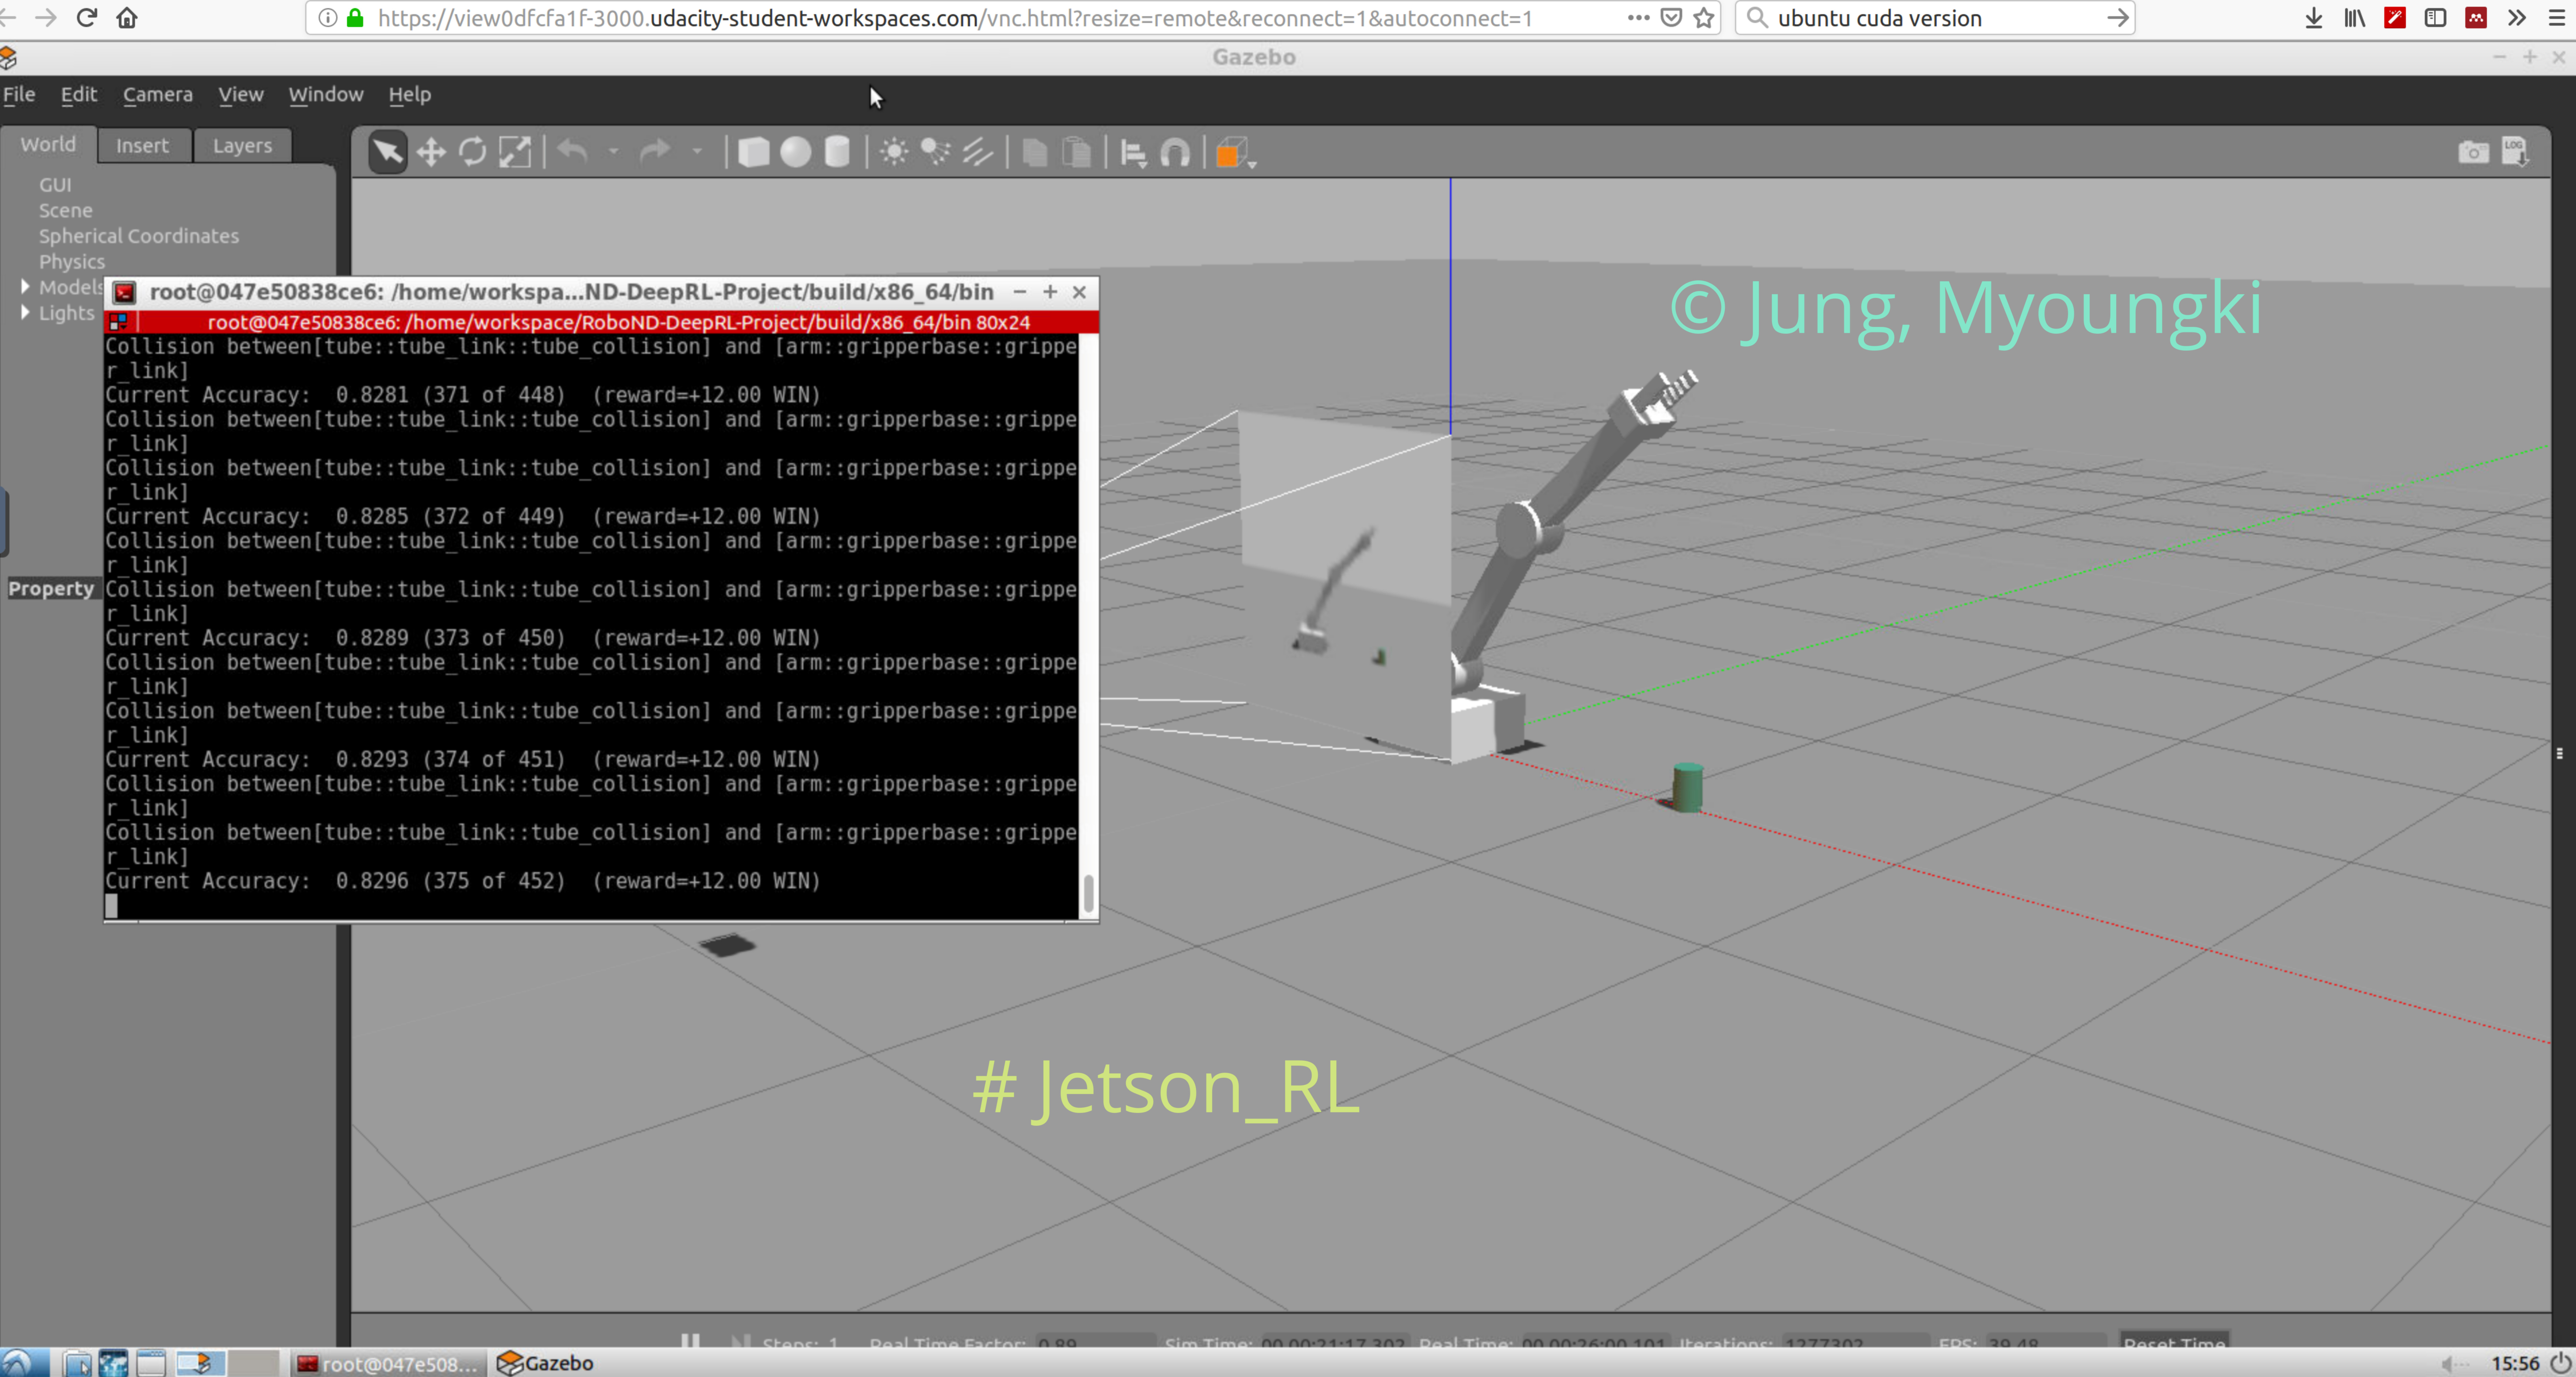
\includegraphics[width=\linewidth]{./img/over80pRLARM.png}
      \caption{Agent reaching overall 80 percent accuracy}
      \label{fig:over80pRLARM}
\end{figure}

200 iterations more the average 90 percent of contact to the tube could be realised, Figure \ref{fig:over90p}, this is above the project requirement. After this point agent's \verb!EPS_END! is 0.05 and rarely starts new exploration in control. Therefore, more than 95 percent of gripper touching the tube could be realised.
\begin{figure}[thpb]
      \centering
      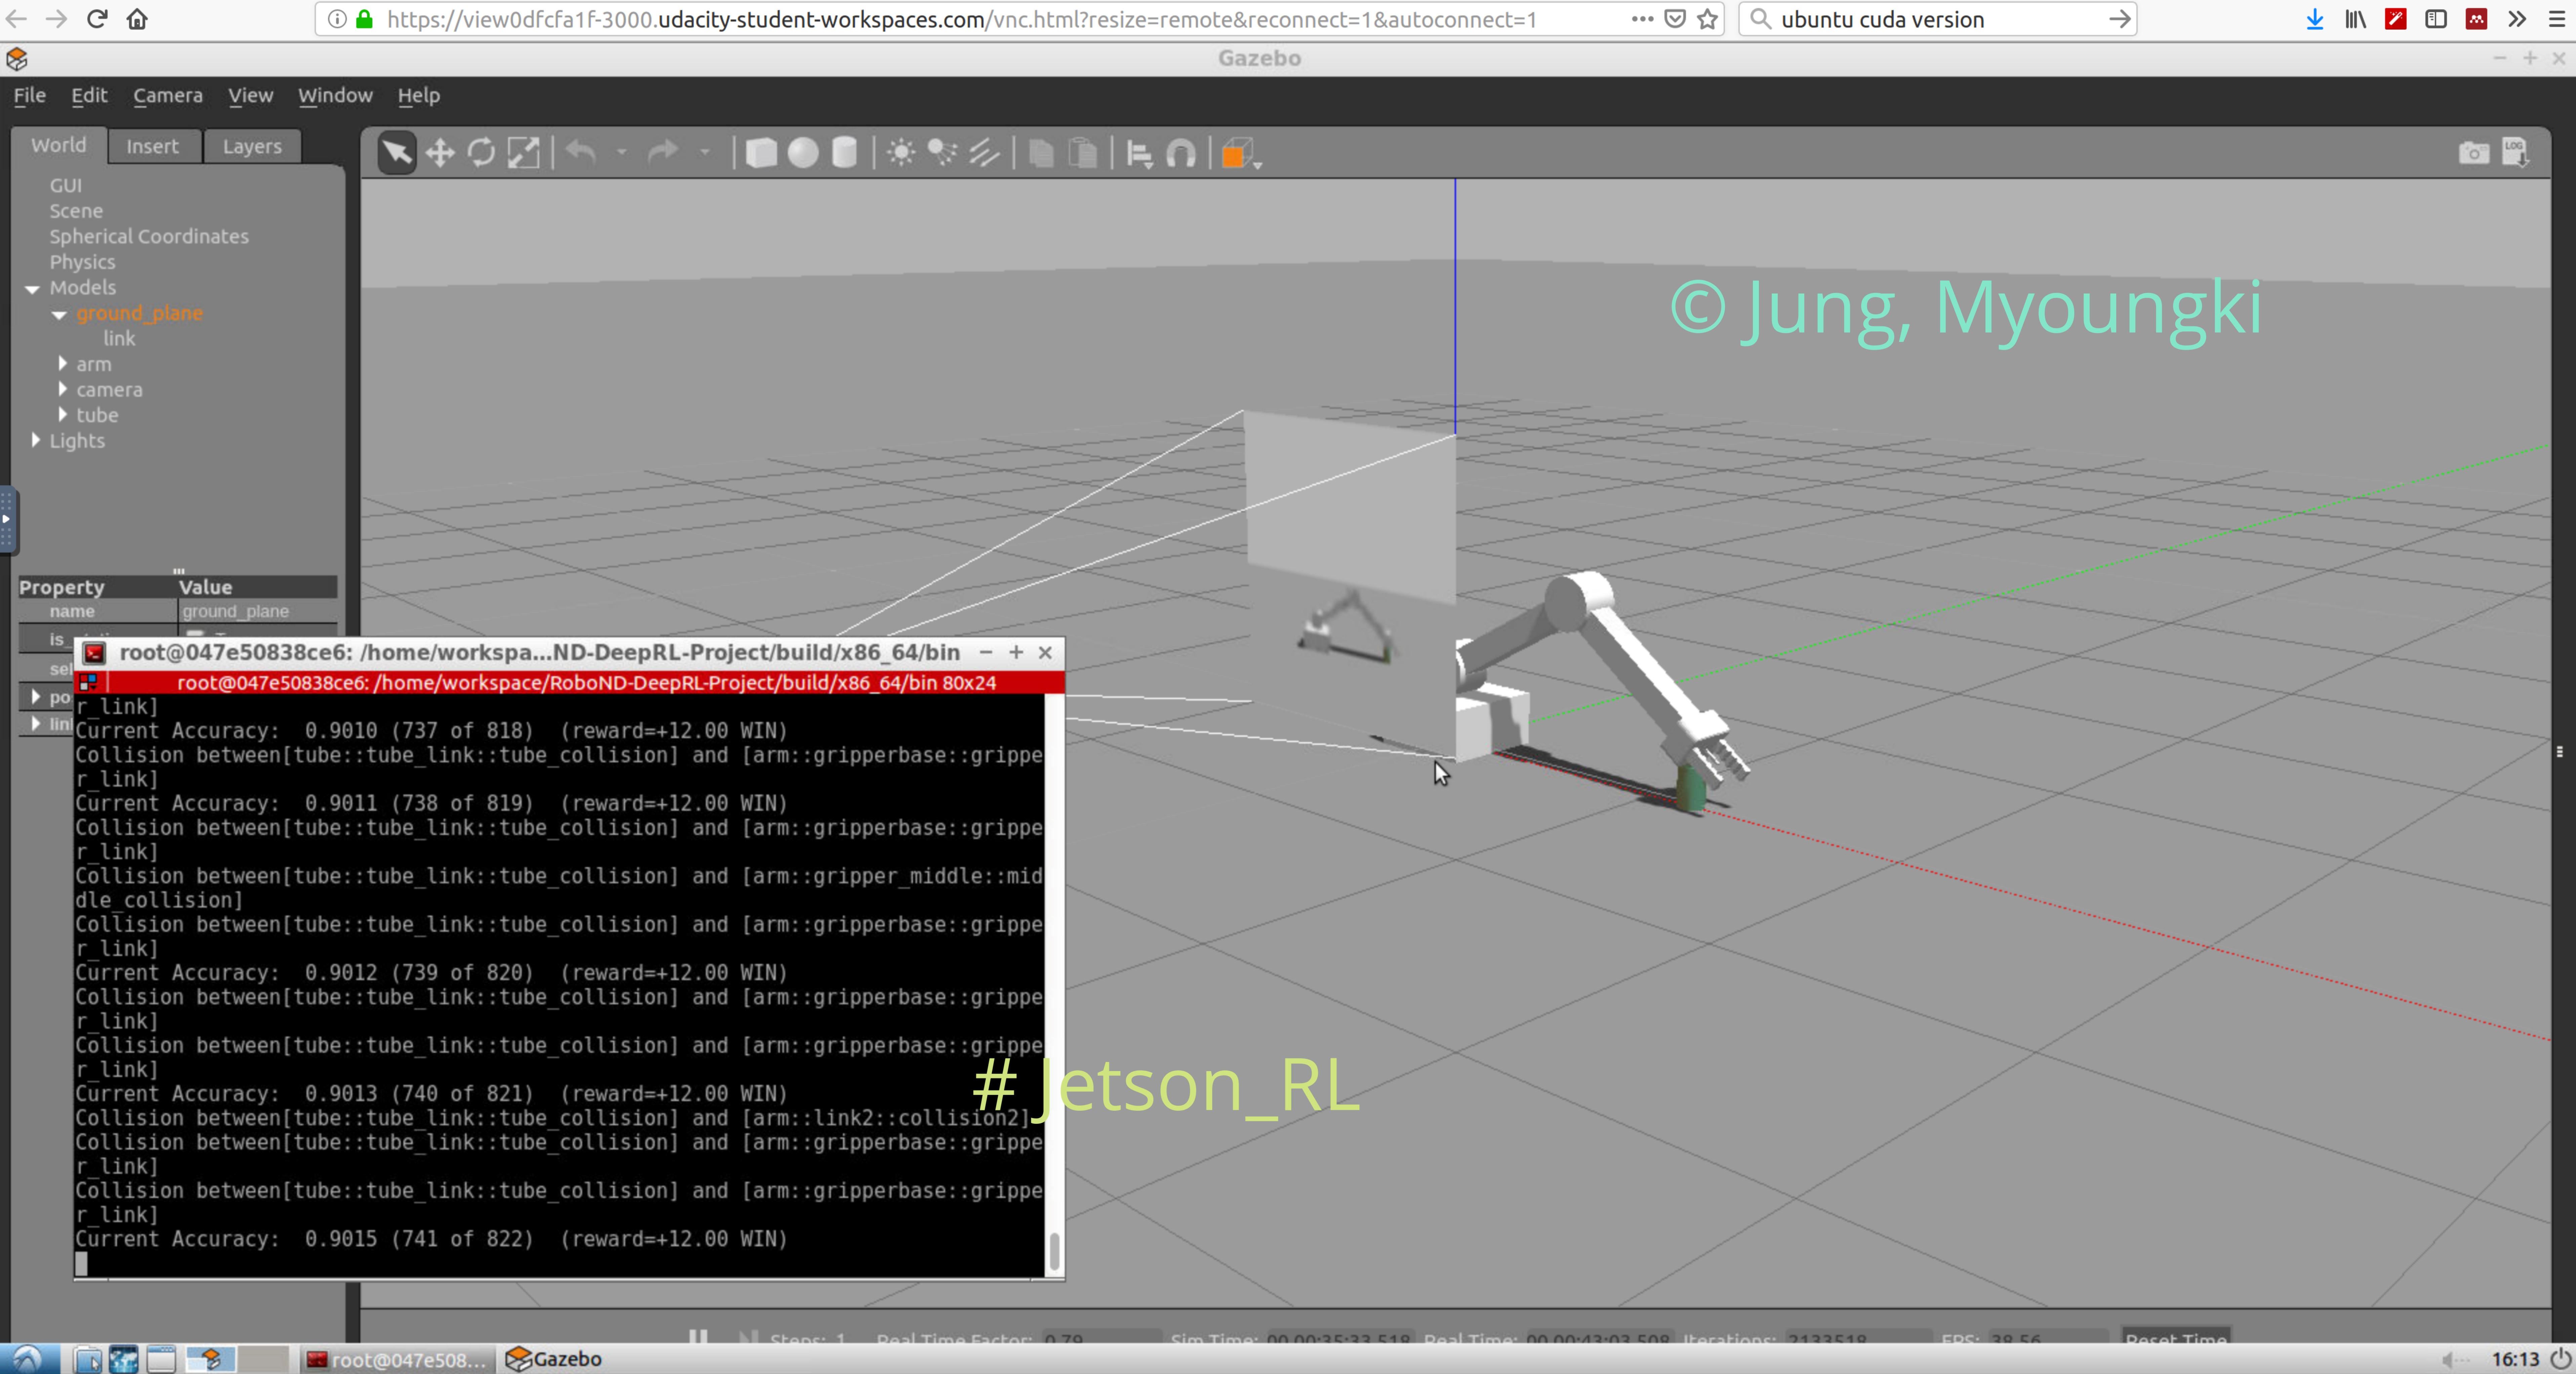
\includegraphics[width=\linewidth]{./img/over90p.png}
      \caption{Agent reaching overall 90 percent accuracy}
      \label{fig:over90p}
\end{figure}

Actual moment of touching the gripper to the tube is snapshoted and shown on Figure \ref{fig:touchingGR86p}.
\begin{figure}[thpb]
      \centering
      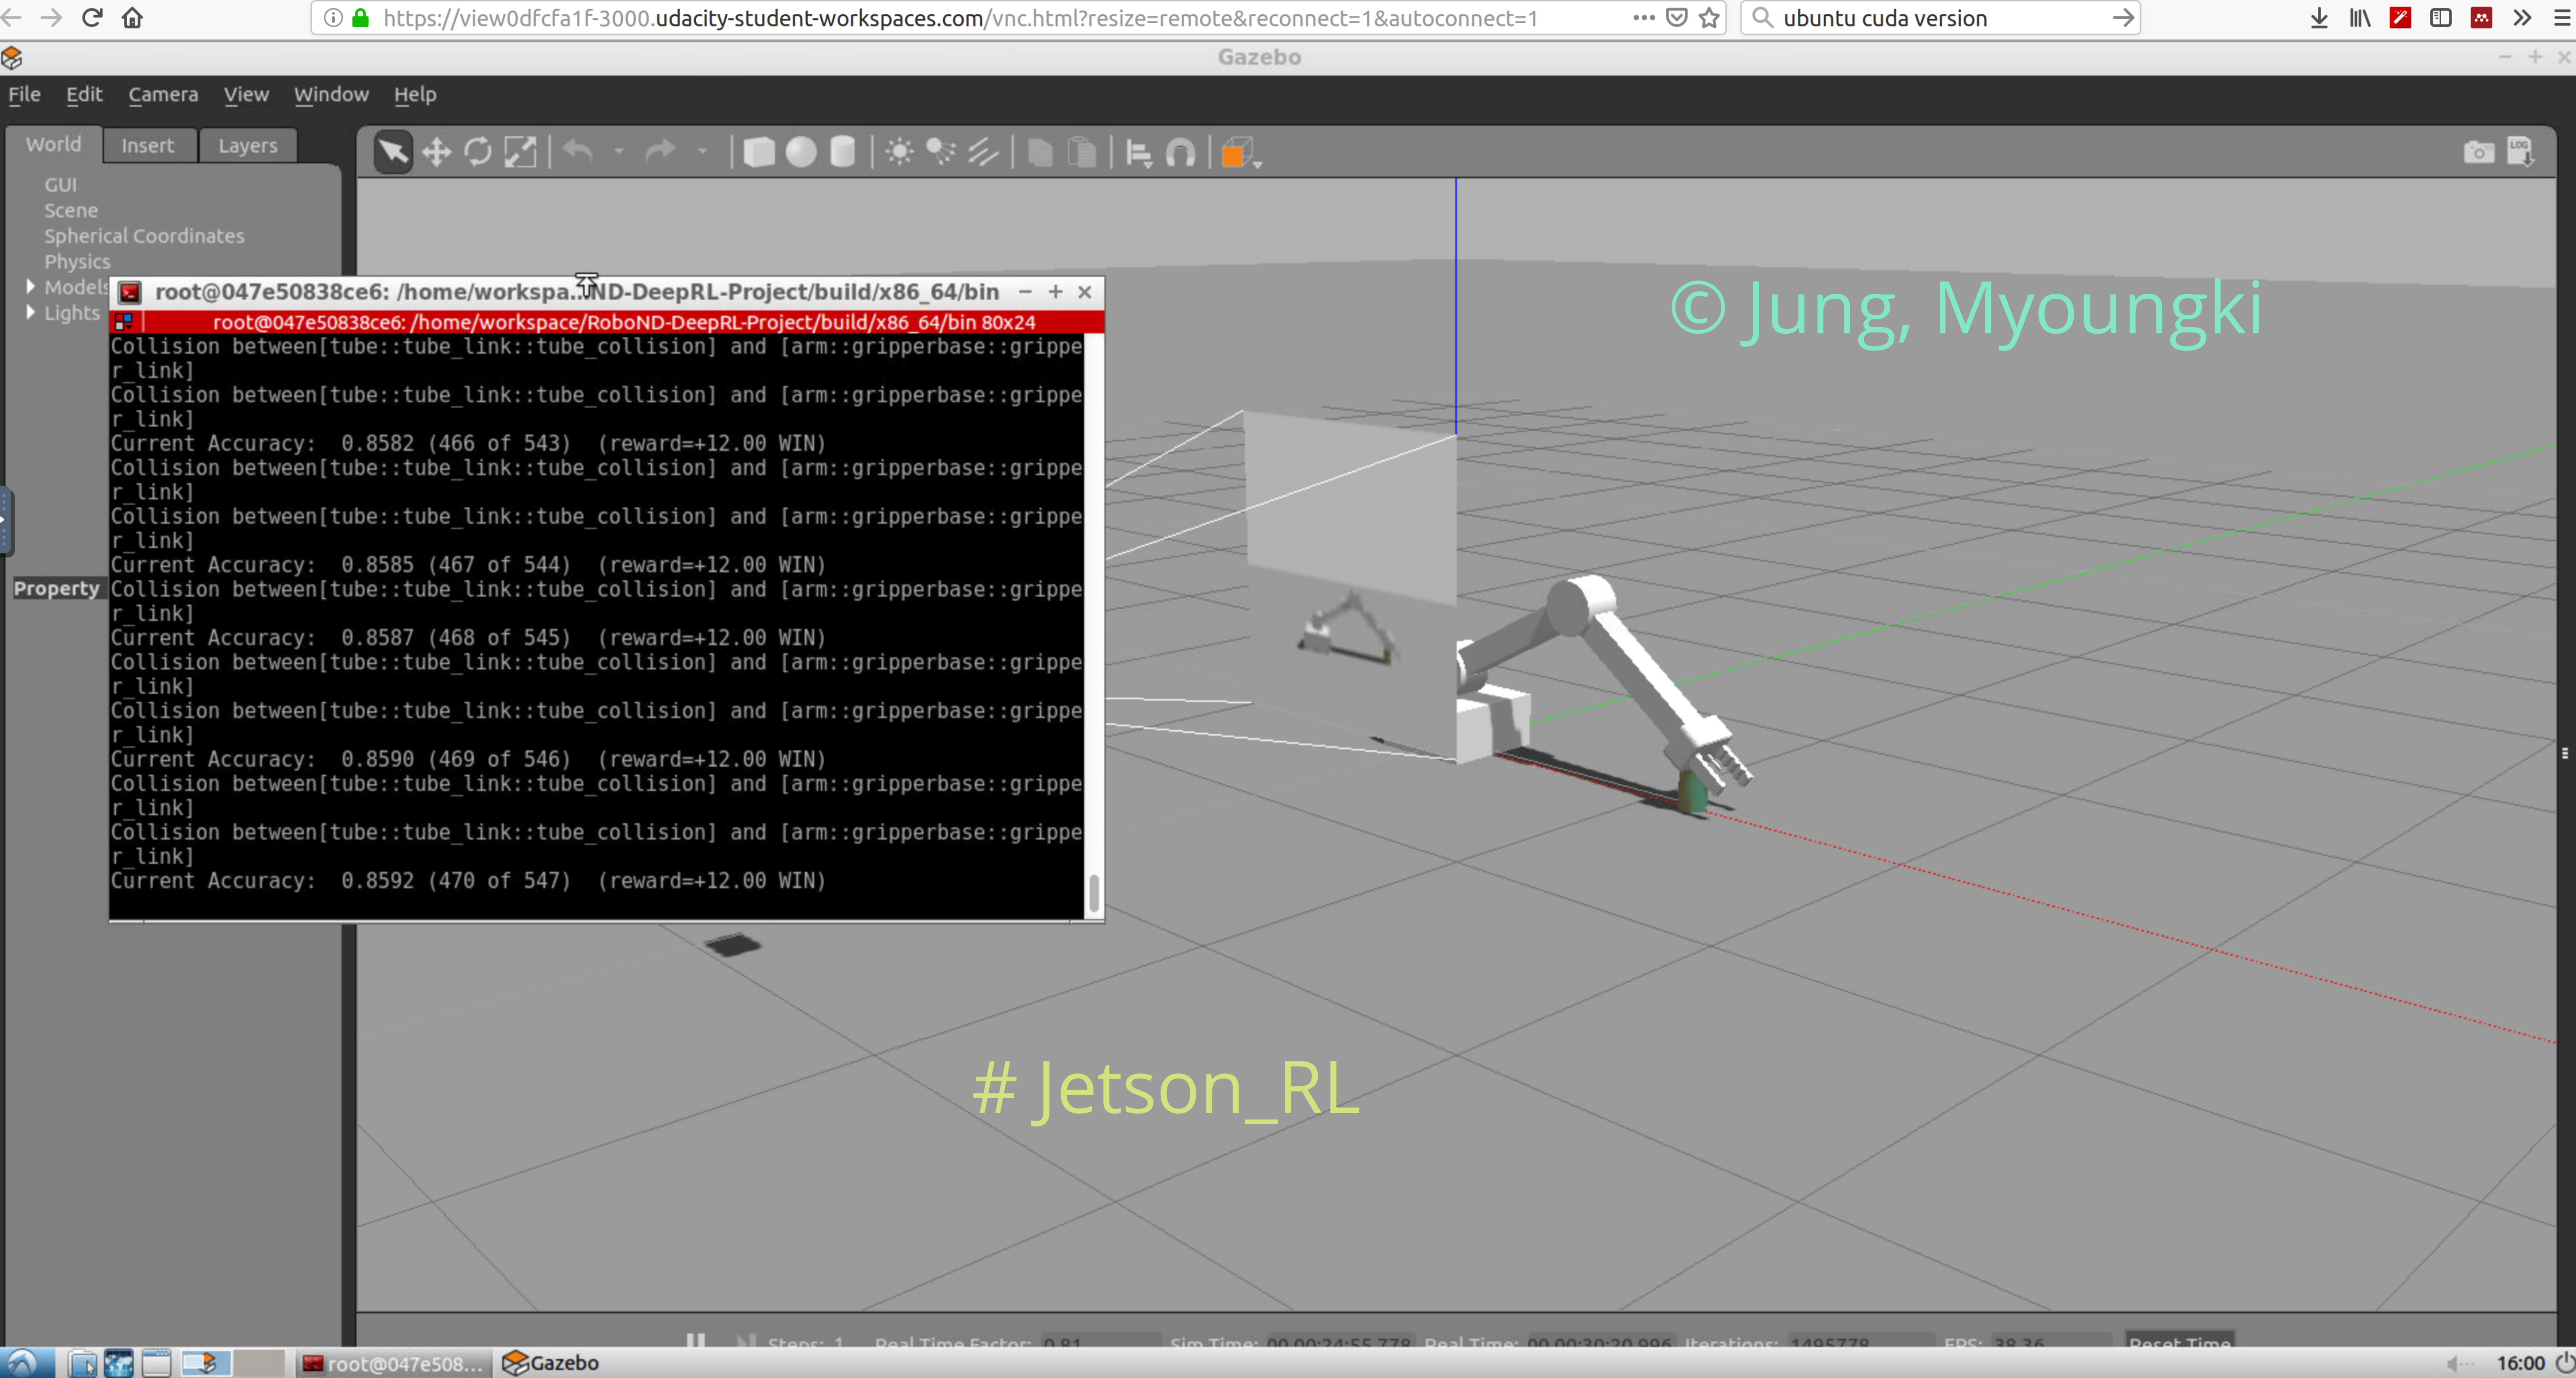
\includegraphics[width=\linewidth]{./img/touchingGR86p.png}
      \caption{Agent reaching reaching with gripper}
      \label{fig:touchingGR86p}
\end{figure}
The videos realated to those images are present in \verb!./Videos! folder of the project.  \verb!./Videos/BeginToLearn.avi! shows struggling agent not knowing what is an expected action. Other videos shows an experienced agens touching the tube confididently, knowing what are actions with rewards over many episodes of learning.
\section{Discussion}
 This experiment shows usage of premade example of jetson reinforcement repository. The building of the libraries of torch was too hard on jetson Xavier, it had to be tested on the udacity workspace, however, some build errors lurks up and had make the environment for the workspace using \verb!sudo apt-get install libignition-math2-dev! to build the \verb!ArmPlugin.cpp!. This repository should be updated for new architectures and prefer not to use a library not readily accessible, pytorch. The backend of the DQN RL could be with tensorflow RT instead of importing python object processed by pytorch, which can be a issue with realtime robot cases by injecting performance issues.
 If saving DQN weights function was implemented it could be better to continue the training after pausing the simulation. Abandonning trained agents' weight every time disconnecting from the workspace seem to be a waste of computing resources and processing time.

 \section{Conclusion / Future work}
The more advanced reinforcement agent algirithms are available. Proximal Policy Optimization Algorithms(PPO) \cite{Schulman2017} is excelent with continous state space and control space like drone flight controller or rocket propulsion control with regard to the continous environmental states. OoenAI foundation suggests Deep deterministic policy gradient (DDPG)\cite{Lillicrap2015} and  Hindsight Experience Replay\cite{Andrychowicz2017},a new experience replay that can learn from failure, as the top of the edge reinforcement learning algorithms and proves their algorithms are outperforming conventional algorithms easily. It is a rapidly developing area of research field. The technology used in this project can be substituted with new algorithms on cutting edge trends.
\bibliography{bib}
\bibliographystyle{ieeetr}

\end{document}
